% uw-wkrpt-se.tex - An example work report that uses uw-wkrpt.cls
% Copyright (C) 2002,2003  Simon Law
% 
% This program is free software; you can redistribute it and/or modify
% it under the terms of the GNU General Public License as published by
% the Free Software Foundation; either version 2 of the License, or
% (at your option) any later version.
% 
% This program is distributed in the hope that it will be useful,
% but WITHOUT ANY WARRANTY; without even the implied warranty of
% MERCHANTABILITY or FITNESS FOR A PARTICULAR PURPOSE.  See the
% GNU General Public License for more details.
% 
% You should have received a copy of the GNU General Public License
% along with this program; if not, write to the Free Software
% Foundation, Inc., 59 Temple Place, Suite 330, Boston, MA  02111-1307  USA
%
%%%%%%%%%%%%%%%%%%%%%%%%%%%%%%%%%%%%%%%%%%%%%%%%%%%%%%%%%%%%%%%%%%%%%
%
% We begin by calling the workreport class which includes all the
% definitions for the macros we will use.
\documentclass[se]{uw-wkrpt}

% LaTeX preamble: load some packages to add functionality
\usepackage{graphicx} % Include graphic importing

\usepackage[T1]{fontenc} % Better fonts
\usepackage{ae,aecompl}

\usepackage{indentfirst} % Indent first paragraph of each section

\usepackage[titletoc,title]{appendix} % Prefix appendix letters with `Appendix'

% For mathematical symbols in our pseudocode
\usepackage{amsmath}

% Use the algorithmicx package for pseudocode
\usepackage{algorithm}
\usepackage{algpseudocode}

% Use biblatex for references
\usepackage[style=ieee,sorting=none,dateabbrev=false,backend=biber]{biblatex}
\addbibresource{uw-wkrpt-bib.bib} % Specify the bibliography file

% This needs to be the last package loaded
\usepackage[pdftex]{hyperref} % Generate PDF links and bookmarks.
\hypersetup{
  bookmarks=true,
  bookmarksnumbered=true
}

% Now we will begin writing the document.
\begin{document}

%%%%%%%%%%%%%%%%%%%%%%%%%%%%%%%%%%%%%%%%%%%%%%%%%%%%%%%%%%%%%%%%%%%%%
%% IMPORTANT INFORMATION
%%%%%%%%%%%%%%%%%%%%%%%%%%%%%%%%%%%%%%%%%%%%%%%%%%%%%%%%%%%%%%%%%%%%%

%% First we, should create a title page.  This is done below:
% Fill in the title of your report.
\title{The Evaluation of ASP.NET Frameworks for Implementing a RESTful OData Service}

% Fill in your name.
\author{Joshua Kalpin}

% Fill in your student ID number.
\uwid{20414492}

% Fill in the name of the PNG file with your signature, or leave unchanged.
\signature{signature}

% Fill in your home address.
\address{109 Serene Way.\\*
         Thornhill, ON\ \ L4J 9A3}

% Fill in your employer's name.
\employer{Microsoft}

% Fill in your employer's city and province.
\employeraddress{Redmond, WA}

% Fill in your school's name.
\school{University of Waterloo}

% Fill in your faculty name.
\faculty{Software Engineering}

% Fill in your student user ID
\userid{jkalpin}

% Fill in your e-mail address.
\email{jkalpin@uwaterloo.ca}

% Fill in your term.
\term{3B}

% Fill in your program.
\program{Software Engineering}

% Fill in the department chair's name.
\chair{Dr.\ A.\ Morton}

% Fill in the department chair's mailing address.
\chairaddress{Software Engineering\\*
              University of Waterloo\\*
	      Waterloo, ON\ \ N2L 3G1}

% If you are writing an "SE-confidential" report, uncomment the next line.
%\confidential{SE-confidential}

% If you want to specify the date, fill it in here.  If you comment out
% this line, today's date will be substituted.
%\date{April 24, 2012}

% Now, we ask LaTeX to generate the title.
\maketitle

%%%%%%%%%%%%%%%%%%%%%%%%%%%%%%%%%%%%%%%%%%%%%%%%%%%%%%%%%%%%%%%%%%%%%
%% FRONT MATTER
%%%%%%%%%%%%%%%%%%%%%%%%%%%%%%%%%%%%%%%%%%%%%%%%%%%%%%%%%%%%%%%%%%%%%
%% \frontmatter will make the \section commands ignore their numbering,
%% it will also use roman page numbers.
\frontmatter

% After this, we must create a letter of submission.
\begin{letter}

I just completed my fourth work term prior to my \theterm{} term. My second work term report, entitled: ``\thetitle'', is attached. My manager was Anandhi Somasekaran within the Azure Active Directory Group at Microsoft. This group was responsible for the identity management APIs and services that powered Active Directory in the cloud.

This report is a comparison between the WebApi and Windows Communication Foundation Data Services (WCF DS) ASP.NET frameworks. These frameworks are the two most commonly used frameworks to create RESTful OData services at a large scale. I worked with both of these frameworks throughout my co-op term to improve the performance of the Azure Active Directory Graph API service.

I have received no direct assistance from anyone on the completion of this report. I wish to thank Anandhi Somasekaran, my manager and Pavan Kompelli, my mentor for their assistance throughout my work term.

% Note that I do not need to type out the boilerplate confirmation,
% nor do I need to write a signature block.  This is generated for me.
% We are now finished with the letter.
\end{letter}

% We continue with required sections, such as the Executive Summary.
\section{Executive Summary}

Microsoft, one of the world's largest software companies, has developed the Azure Active Directory Graph API service to allow developers to create applications that leverage their Active Directory instances. This service was originally developed in 2012 using the ASP.NET Windows Communication Foundation Data Services (WCF DS) framework with the Open Data (OData) protocol. At the time, the WCF DS framework was the only option for building an OData service.

As the Graph API service matured, performance issues began to arise. When the service received large amounts of concurrent requests, response rates would decrease, CPU usage would spike on servers and performance in general would degrade. These issues were making it difficult to scale the service for more customers and were blocking a number of potential customers from using the service.

This report compares the WCF DS framework to a new framework called WebApi for building a RESTful OData service on performance, code quality and the ability to add new OData features. WebApi is a Model-View-Controller based framework and has become the recommended framework for developing OData services. It also supports the latest version of the OData protocol, which WCF DS does not.

Both frameworks perform on a similar level in terms of average request speed and CPU usage. However, the WebApi framework supports the OData select operation, which allows developers to choose which properties they want on objects. When this operation is used, the average request time drastically increases and CPU usage drops. In terms of code quality the WebApi framework is much easier to understand and uses significantly less code to accomplish its tasks.

In the end, the analysis indicates that the WebApi framework is much better for building RESTful OData services than the WCF DS framework. With the select feature, WebApi performs much better, has better code quality and supports the latest version of OData. This report highly recommends that anyone developing a RESTful OData service using ASP.NET should use the WebApi framework.

% Next, we need to make a Table of Contents, List of Figures and 
% List of Tables.  You will most likely need to run LaTeX twice to
% get these correct.  The first pass for LaTeX to figure out the
% labels, and the second pass to put in the right references.
\tableofcontents
\listoffigures
\listoftables

%%%%%%%%%%%%%%%%%%%%%%%%%%%%%%%%%%%%%%%%%%%%%%%%%%%%%%%%%%%%%%%%%%%%%
%% REPORT BODY
%%%%%%%%%%%%%%%%%%%%%%%%%%%%%%%%%%%%%%%%%%%%%%%%%%%%%%%%%%%%%%%%%%%%%
%% \main will make the \section commands numbered again,
%% it will also use arabic page numbers.
\mainmatter

% You must have an Introduction
\section{Introduction}\label{sec:intro}

Microsoft is one of the largest software companies in the world that develops devices and services for both consumers and enterprises. The company's products can be found all over the world and are used by millions of people every day. In May 2014, the author of this report joined the Azure Active Directory (AAD) group within the Cloud and Enterprise (C \& E) division of Microsoft. Within this group the author was on the AAD Graph team. This team is responsible for developing the service that powers the AAD Graph API. The API allows developers to create applications to interface with a company's Active Directory instance. The AAD Graph API is one of Microsoft's most used services and is relied upon by a large portion of the company.

Active Directory is "a special-purpose database" that is "designed to handle a large number of read and search operations"~\cite{ref:ad}. The primary use of Active Directory is to allow organizations to manage their organizations. See figure \ref{fig:ad} for a visual example of a directory.

\begin{figure}
  \centering
  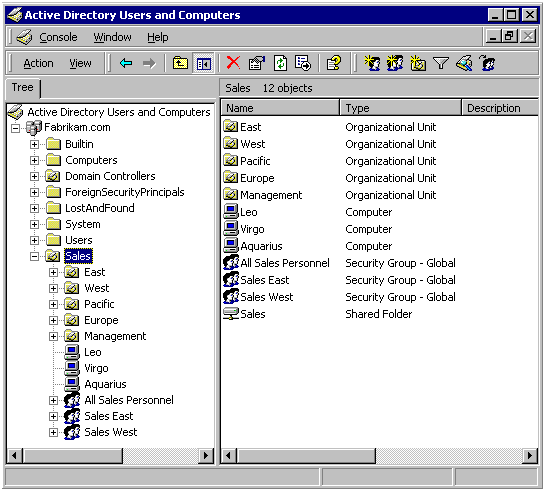
\includegraphics[height=3.5in]{ad}
  \caption[An example directory in Active Directory.]{An example directory in Active Directory.}~\cite{ref:ad}
  \label{fig:ad}
\end{figure}


When the API was first released in 2012, it was implemented using the ASP.NET Windows Communication Foundation Data Services (WCF DS) framework with support for the Open Data (OData) protocol~\cite{ref:graph}. This protocol allows for queries to completed with url requests. This includes filtering, sorting and paging responses. At the time, this framework was the only option for creating a service that supported the OData protocol.

As the service matured with the WCF DS framework, performance, code quality and complications with adding more OData features began to arise. Additionally, the ASP.NET team officially deprecated the WCF DS framework in 2014 in favour of a new Model-View-Controller based framework called WebApi~\cite{ref:wcfds}. In May 2014 an investigation began into replacing the WCF DS framework within the Graph API.

There are a number of objectives of replacing the WCF DS framework. First, there should be a noticeable performance increase to the service. Specifically, the service should be faster and use less CPU. Second, the code quality of the service should improve. Third, it should be easy to add more OData features to the service. Last, the service should be able to support the newest version of OData, version 4. 

This report compares the WCF DS and WebApi frameworks for implementing a RESTful OData service. The analysis will include performance numbers, code quality and scalability concerns. These findings were determined during the investigation and subsequent implementation of the Graph API using WebApi. The performance comparisons are between the new version of the service and the service that is currently running in production. This report is intended for those who wish to implement an OData service, are converting a WCF DS service to use WebApi or those interested in building a scalable distributed service using ASP.NET.

The reader should have a background in building web services and software development. It will be helpful for the reader to know ASP.NET, C\#, and how to develop software on the Microsoft platform.

\section{Background}

The original Graph API service is based on the ASP.NET WCF DS framework. When the service was created, this was the only ASP.NET framework that supported the OData protocol. The WCF DS framework uses an interface design pattern that requires developers to implement a series of interfaces to handle different types of requests. This includes GET, POST, PATCH, and DELETE requests.

In the two years since the development of the original Graph API service, a new ASP.NET framework called WebApi, was developed and replaced WCF DS as the primary framework for building OData services. This framework is based off the the Model-View-Controller (MVC) design pattern (figure \ref{fig:mvc}), instead of an interface based design. WebApi handles a majority of the request routing, serialization and the creation of responses. Due to the proliferation of WebApi, WCF DS was subsequently deprecated and all development has ceased.


\begin{figure}
  \centering
  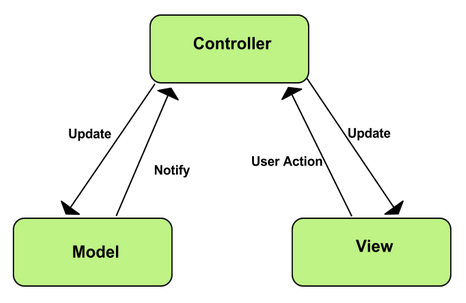
\includegraphics[height=3in]{mvc}
  \caption[A flow diagram for the Model View Controller design pattern.]{A flow diagram for the Model View Controller design pattern.}~\cite{ref:mvc}
  \label{fig:mvc}
\end{figure}

\subsection{The Open Data Protocol}

The Open Data protocol (OData) "is a standardized protocol for creating and consuming data APIs" that was developed by Microsoft~\cite{ref:odata}. The protocol has a number of features that make it easy for APIs to support queries that are similar to SQL. OData version 3, the latest version that is supported by the Graph API, supports querying collections, requesting individual objects, getting relationships between objects, and the number of objects that exist. Relationships can be one-to-one (one object to another) or many-to-one (one object linked to a collection of objects).

For querying collections, OData supports multiple operations including filtering, selecting, ordering, selecting page size, skipping a certain number of objects, and choosing what format to return a request in. Filtering allows a user to pick requirements that the returned objects must have. Selecting allows users to choose which properties are returned from objects in the response. The page size is the maximum number of objects that can be returned in a request response. Skipping allows a user to skip a certain number of objects and return the subsequent ones in the response. Formatting allows for results to be returned in various forms of JSON or XML. The Graph API currently supports a subset of these operations. This subset does not include the select operation which will be elaborated on in section \ref{subsec:issues} and section \ref{subsec:req}.

In the future, the Graph API will need to support the latest version of the OData protocol, released in March 2014~\cite{ref:odatav}. This version of the protocol is not backwards compatible with previous versions and adds more operations for querying collections.


\subsection{Current Issues}\label{subsec:issues}

The current version of the Graph API service has experienced a number of issues. These issues range from performance, to code quality, to the ability to add new features.

In terms of performance issues, the service runs into problems when it receives a large amount of concurrent request. Individual requests will take longer, and large requests can take multiple seconds to complete. CPU use will also spike. This makes it difficult to scale the service up inexpensively.

In terms of code quality issues, the interface design pattern that WCF DS uses makes it difficult for new programmers to understand how the system functions. It is challenging to determine where requests first hit the service and how responses are returned to users. This has caused new members of the AAD Graph team to spend a significant amount of time learning the system before being able to contribute to the team.

The ability to add features is one of the largest roadblocks for scaling and adding features to the Graph API service. The current service does not support the select operation in the OData protocol. This feature would allow users of the API to choose which properties are returned from objects in responses. For example, if object A has five properties, a developer can choose to select the two properties that are needed for the application. Implementing this feature in the current service would be incredibly difficult, even though it is of high value.

\section{Analysis}

\subsection{Requirements}\label{subsec:req}

Any replacement to the current Graph API service has to fulfill a number of requirements. These are mandatory and if they are not met the current service will not be replaced.

The first requirement is that there must not be any performance decreases with the new service. This means that the service must be not process requests slower or use more CPU. 

The second requirement is that the code quality must improve. In an ideal situation the new version of the service must be easier to understand and easier for new team members to get on-boarded. This requirement may also include reducing the number of lines of code and code duplication in the service as well.

The third requirement is that the new service must be able to support the OData select operation. This requirement is tied in with the performance improvements because a request with the select operation is expected to be smaller. A smaller request is faster to process and uses less CPU, making it easier to scale the service. This has also been a request from a number of users of the API since its creation.

The last requirement is that the new service must be able to support OData version 4. This is required for future growth of the service and future internal projects that will use the service. Additionally, the current service will never be able to support this requirement, so it is mandatory for any replacement.

\subsection{Evaluation Criteria}

To decide which framework, WebApi or WCF DS, is the most suitable for the Graph API service a number of evaluation criteria were used. On the quantitative side, the average request speed and CPU usage while getting 100 objects and getting 999 objects are compared. The ability to add new features will also be compared by evaluating the length of time that it takes to implement the select feature in the service.

On the qualitative side, the code quality between the two services will be compared. The complexity of the two designs will also be compared. This comparison will be done by polling the members of the AAD Graph team and by manual inspection. The ability to support OData version 4 will not be directly compared, as WCF DS does not currently support it.

The quantitative criteria will be weighed significantly more than the qualitative criteria. This is because the performance and scalability requirements are more important than the code quality ones.

\subsection{Experimental Procedure}\label{subsec:proc}

The procedure for obtaining the test results for each service was identical. A Python script was used to make requests to the server that was running the services. This script made 2000 requests to the WebApi service and then 2000 requests to the WCF DS service. For each request the script stored the current computer time, executed the request, recorded the computer time and then stored the difference to determine how long the request took to complete.

The results for CPU usage were obtained by running the Performance Monitor program that came with Windows Server 2008 while the script ran. The program works by polling CPU usage for the processor and specific processes. The result is then stored as a graph that can be exported for later use. 

\subsection{Results}

There are two categories of results that can be obtained from testing the two services: performance and code quality. The performance results compare requests to the WebApi service, WCF DS service, and the WebApi service with only five properties selected. WCF DS has no results for select because it does not support the operation. The code quality results compare the readability and understandability of the code qualitatively.

\subsubsection{Speed}

After running the testing script (see section \ref{subsec:proc}) results were obtained. The averages, standard deviations, maxima, and minima are shown in table \ref{tbl:100speed} for 100 objects, and table \ref{tbl:999speed} for 999 objects. 

\begin{table}
  \caption{100 Objects - Request Speed in Seconds}
  \label{tbl:100speed}
  \centering
    \begin{tabular}{ | l | l | l | p{5cm} |}
    \hline
     & \textbf{WCF DS} &  \textbf{WebApi} & \textbf{WebApi Select} \\ \hline
    \textbf{Average} & 0.277 & 0.268 & 0.164 \\ \hline
    \textbf{Standard Deviation} & 0.018 & 0.016 & 0.014 \\ \hline
    \textbf{Maximum} & 0.386 & 0.333 & 0.233 \\ \hline
     \textbf{Minimum} & 0.216 & 0.201 & 0.116 \\
    \hline
    \end{tabular}
\end{table}

For 100 objects, the WebApi service is on average 9 milliseconds (ms) than WCF DS. Its maximum request time is 50 ms faster than the WCF DS service and the WebApi service's fastest request was 15 ms faster. From these results, there is no major difference between the two services. However, when the WebApi service's select operation is used, the difference is noticeable. The average request time for WebApi select is over 100 ms faster than both the WCF DS service and WebApi service with regular requests. Its maxima and minima are also 100 ms faster. The standard deviation for all results is within an acceptable range for the numbers.

\begin{table}
  \caption{999 Objects - Request Speed in Seconds}
  \label{tbl:999speed}
  \centering
    \begin{tabular}{ | l | l | l | p{5cm} |}
    \hline
     & \textbf{WCF DS} &  \textbf{WebApi} & \textbf{WebApi Select} \\ \hline
    \textbf{Average} & 1.92 & 1.75 & 0.600 \\ \hline
    \textbf{Standard Deviation} & 0.322 & 0.594 & 0.219 \\ \hline
    \textbf{Maximum} & 6.93 & 6.88 & 5.42 \\ \hline
     \textbf{Minimum} & 1.42 & 1.35 & 0.435 \\
    \hline
    \end{tabular}
\end{table}

For 999 objects, the WebApi service is 170 milliseconds (ms) faster than the WCF DS service. WebApi's maximum request time is 50 ms faster than WCF DS and its minimum time is 70 ms faster. Similar to the 100 object request, the WebApi service's select performs significantly better than both WCF DS and regular WebApi requests. With the larger payload, this effect is magnified to be approximately 300\% faster than the other two request types. The standard deviation for this test was higher than the 100-object test, but it is still within an acceptable range.

These results show that the WebApi service performs marginally faster than WCF DS service when requesting 100 objects and 999 objects. However, when selecting five properties with the WebApi service, the service performs three times as fast as the WCF DS service.

\subsubsection{CPU Usage}

CPU usage was measured while running the script that measured average speed (see section \ref{subsec:proc}). This data was gathered by the Perfmon tool and recorded as a graph. Data for both the 100-object test and the 999-object test were obtained and are shown in figure \ref{fig:100cpu} and figure \ref{fig:999cpu}.

The way that Perfmon displays CPU usage is on a scale from 0 to 100 percent. In both charts, the green line represents the total CPU usage on the server. The blue line represents the percent of the total CPU usage that the WebApi service is using. The olive line represents the percent of the total CPU usage that the WCF DS service is using. The first blue section is the WebApi service with all properties select and the second section is the WebApi service with five properties selected. Any significant dips in CPU usage in the graphs (specifically the WCF DS section in figure \ref{fig:100cpu}) can be ignored and are unrelated to the test.

\begin{figure}
  \centering
  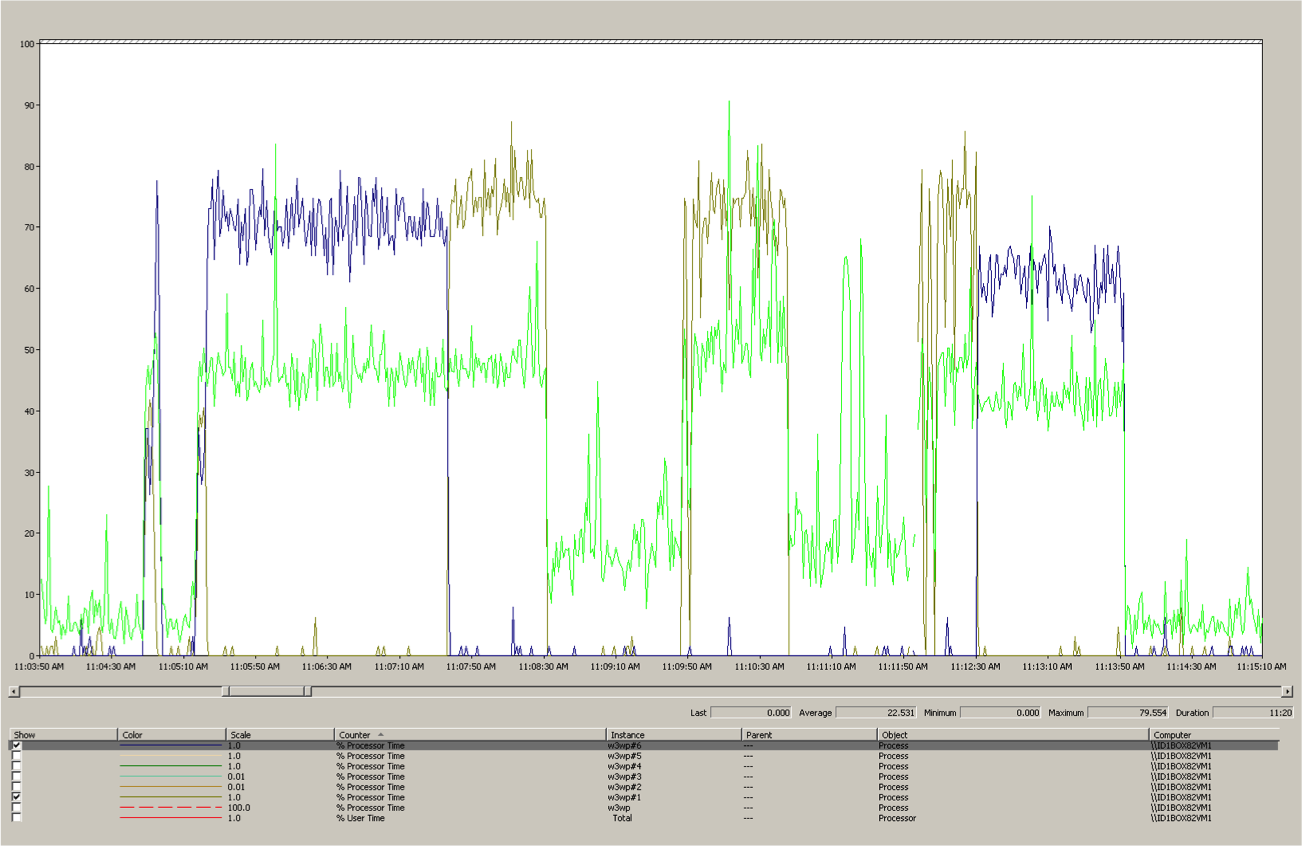
\includegraphics[height=3in]{100CPU}
  \caption{The CPU usage chart for requesting 100 objects}
  \label{fig:100cpu}
\end{figure}

In the 100 object test (see figure \ref{fig:100cpu}), the WebApi service and the WCF DS service use approximately 80\% of the total CPU usage on the server. The total CPU usage sits at approximately 50\% throughout both tests. The difference is impossible to determine between the two services. The WebApi service with five properties selected, which is the second blue area, uses approximately 70\% of the total CPU on the machine. The total CPU usage is at approximately 45\%, around 5\% lower.

\begin{figure}
  \centering
  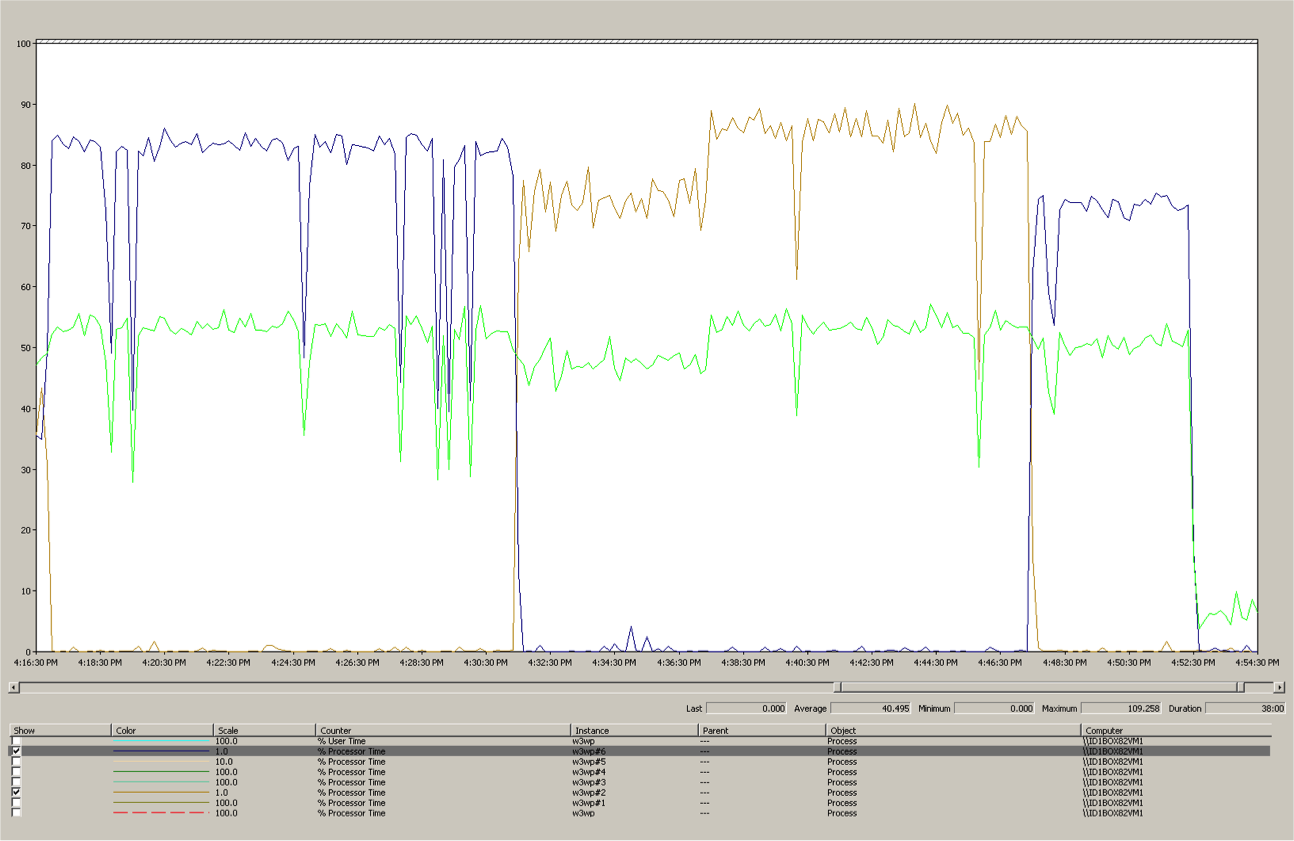
\includegraphics[height=3in]{999CPU}
  \caption{The CPU usage chart for requesting 999 objects}
  \label{fig:999cpu}
\end{figure}

In the 999 object test (see figure \ref{fig:999cpu}), the WebApi service and the WCF DS service use approximately 85-90\% of the total CPU usage on the server. There is a section of the WCF DS test that uses less CPU than the WebApi service and another section that uses more. The total CPU usage for both WCF DS and WebApi is approximately 55\%. Similar to the 100 objects test, when it is averaged out, the difference is almost non-existent. The WebApi service with five properties selected uses approximately 75\% of the total CPU usage. However, the total CPU usage for the server remains around 55\%.

\subsubsection{Code Quality}

Code quality was measured in two different ways. First, the development team for the AAD Graph API was asked which design they felt was easier to understand and less complicated. Second, the number of lines of code and classes required to complete various operations in the service were compared qualitatively.

The ten members of the AAD Graph team were asked to compare the current service using WCF DS to the new version of the service running WebApi on code quality and design. Eight of the members on the team felt that the WebApi service design was much simpler and easier to understand. Additionally, they felt that it would be easier to add new features to the WebApi service and it would be easier for new members of the team to become familiar with if the service were to be fully implemented. The other two members cited familiarity with the existing service and that they felt that WebApi was too difficult to customize.

Comparing the lines of code between the two projects, the WebApi service used significantly less code to perform similar operations when compared to the WCF DS service. There were also fewer files that were specific to the WebApi implementation or that had dependencies on WebApi.

\section{Experimental Errors}

There were a number of areas that experimental errors and places bias could have occurred. These center mainly on the environment that the tests were run in and that the developer of the WebApi version is the author of this report.

During all tests there were other processes running on the server that both the WCF DS and WebApi services were running on. These processes could have affected the performance of both of the services and the speed of the server. This would have also skewed the results recorded by Perfmon too.

Network latency could have also affected the results of the tests. The two machines used in the tests were in a similar location, but the tests did not take into account network latency when measuring the response times. This would have had a larger effect on the 999-object test, as the request response was significantly larger than the 100 object one.

% You must have a Conclusions section
\section{Conclusions}

The initial performance results indicate that there is no real improvement when using the WebApi framework over the WCF DS framework for building a RESTful OData service. Both the average request time and CPU usage are not different enough to declare one better over the other. The main difference occurs when the WebApi service is using select operation.

Using the select operation results in requests being completed 200\% faster for 100\% objects and 300\% faster for 999 objects. For CPU usage, this results in approximately a 5\% drop in overall CPU usage. While this is not a large amount, it is still an improvement. Since implementing select in WCF DS has so far proven nearly impossible, and only took a short amount of time to complete in WebApi, WebApi edges out WCF DS in terms of performance. The ability to let users of the API choose what properties they want on objects puts the performance implications in their hands and results in less load on the server.

In terms of code quality, WebApi wins by a large margin. Based on feedback from the AAD Graph team and the proliferation of the Model-View-Controller design pattern in industry, WebApi is much easier for developers to understand. The amount of code required to complete tasks is much smaller and the code is much simpler.

The other quality about WebApi is that it is still actively being developed and supported. The ASP.NET team has deprecated the WCF DS framework and new features are no longer being developed. This blocks any future support for OData version 4 as well as any performance improvements that come along with new versions of the library.

Based on performance it is impossible to determine whether the WebApi framework is better than the WCF DS framework. However, when factoring in the performance gains from using select, the code quality improvements and the ability to support the latest version of OData, WebApi is the appropriate framework to use for the AAD Graph API service.

% You must have a Recommendations section
\section{Recommendations}

This report recommends that anyone who wants to build a RESTful OData service using ASP.NET should use the WebApi framework over the WCF DS framework. The ability to quickly implement new OData features, especially select, makes it easier to scale and expand a service. WebApi is also the currently supported method of creating OData services while WCF DS is deprecated.

It is also recommended that the AAD Graph API service should continue to be converted over to using the WebApi framework. The support for OData version 4 and select are essential for the service to grow within and outside of the company.

To attempt to increase performance out of WebApi, the OData and WebApi teams should allow for significantly more customization. This includes the ability to profile the service to determine where performance issues occur. The ability to disable certain features and validations that could lead to performance issues should also be added.

To ensure that the service will perform at its optimal capacity a performance optimization engineer should be enlisted to assist in scaling and optimizing the service. Using a different framework will only improve performance to a certain amount. Fine-tuning of the code that does not depend on the framework will also be needed.

%%%%%%%%%%%%%%%%%%%%%%%%%%%%%%%%%%%%%%%%%%%%%%%%%%%%%%%%%%%%%%%%%%%%%
%% BACK MATTER
%%%%%%%%%%%%%%%%%%%%%%%%%%%%%%%%%%%%%%%%%%%%%%%%%%%%%%%%%%%%%%%%%%%%%
%% \backmatter will make the \section commands ignore their numbering,
\backmatter

% Here, we insert a References section, which will be formatted properly.
% The list of works you have referenced should be specified in the preamble.
% In this template, the file is uw-wkrpt-bib.bib.
%
% Note, you will need to process the document in a certain order.  First,
% run LaTeX.  The % first pass will allow LaTeX to build a list of 
% references, it may % emit warning messages such as:
%   LaTeX Warning: Reference `app:gnugpl' on page 4 undefined on input line 277.
%   LaTeX Warning: There were undefined references.
% This is normal.  Now you run BiBTeX in order to generate the proper
% layout for the references.  After this, you run LaTeX once more.
\printbibliography[heading=bibintoc]

\section{Acknowledgements}
% This section shall acknowledge the people who helped with the writing 
% of the work report. This would include anyone who was interviewed, 
% anyone who proofread the report, or anyone whose files were used in 
% the writing of the report.
I would like to thank the Azure Active Directory Graph team for all the feedback during the completion of this project and guidance on this report.

I used the \textsf{uw-wkrpt} document class written by Simon Law to 
typeset it.

\end{document}
